\documentclass[12pt,a4paper]{report}

\usepackage[T1]{fontenc}
\usepackage{graphicx}
\usepackage{url}
\usepackage{setspace}
\usepackage{times}
\usepackage{hyperref}
\usepackage[nottoc,notlot,notlof]{tocbibind}
\usepackage{amsmath}
\usepackage{amssymb}
\usepackage{caption}
\usepackage{subcaption}
\usepackage{booktabs}
\usepackage{array}
\usepackage{tikz}
\usepackage{pgfplots}
\pgfplotsset{compat=1.18}
\usetikzlibrary{shapes.geometric, arrows, arrows.meta, positioning, fit, backgrounds, calc}
\usepackage[left=3.5cm,top=2cm,right=3cm,bottom=4cm]{geometry}
\setcounter{tocdepth}{2}

\renewcommand{\baselinestretch}{1.25}
\renewcommand{\bibname}{References}
\renewcommand\listfigurename{\centering{List of Figures}}
\renewcommand\listtablename{\centering{List of Tables}}


%% ---- TikZ styles ----
\tikzstyle{process}   = [rectangle, rounded corners, minimum width=3.2cm, minimum height=1cm,
                          text centered, draw=black, fill=blue!15, text width=3cm]
\tikzstyle{entity}    = [rectangle, minimum width=2.8cm, minimum height=1cm,
                          text centered, draw=black, fill=orange!20, text width=2.6cm]
\tikzstyle{datastore} = [rectangle, minimum width=3cm, minimum height=0.8cm,
                          text centered, draw=black, fill=yellow!25,
                          double, double distance=2pt, text width=3cm]
\tikzstyle{arrow}     = [thick,->,>=stealth]
\tikzstyle{darrow}    = [thick,<->,>=stealth]

\begin{document}

%% ============================================================
%%  TITLE PAGE
%% ============================================================
\begin{titlepage}
\begin{center}
{\LARGE \textbf{Physical Injury Risk Prediction in Sports\\[0.2cm] Using Machine Learning}}\\[0.2cm]
\vspace{1cm}
{\Large \textbf{A Mini Project Report}}\\
\vspace{0.4cm}
\large \textit{Submitted to the APJ Abdul Kalam Technological University}\\
\vspace{0.1cm}
\large \textit{in partial fulfillment of requirements for the award of degree}\\
\vspace{0.8cm}
{\Large \textbf{Bachelor of Technology}}\\
\vspace*{0.1cm}
\large{in}\\
\vspace*{0.1cm}
{\Large \textbf{Computer Science and Engineering}}\\
\vspace*{0.1cm}
\large \em{by}\\
\vspace*{0.1cm}
{\Large \textbf{\scshape{Lathika}}}({\textbf{B23CSXXXX, KTU Reg No: }})\\
{\Large \textbf{\scshape{Sijo}}}({\textbf{B23CSXXXX, KTU Reg No: }})\\
{\Large \textbf{\scshape{Gokul}}}({\textbf{B23CSXXXX, KTU Reg No: }})\\
{\Large \textbf{\scshape{Aswin}}}({\textbf{B23CSXXXX, KTU Reg No: }})\\
\vspace*{1cm}
\centerline{
\includegraphics[width=5cm]{logo.png}}
\vspace*{-1cm}
\begin{center}
  {\bf \large Department of Computer Science and Engineering}\\
  {\bf \large Mar Baselios College of Engineering and Technology (Autonomous)}\\
  {\bf \large Mar Ivanios Vidya Nagar, Nalanchira}\\
  {\bf \large Thiruvananthapuram--695015}\par
  \vspace{0.3cm}
  {\bf \large April 2026}\\\par
\end{center}
\vfill
\end{center}
\end{titlepage}
\pagebreak
\pagenumbering{gobble}

%% ============================================================
%%  CERTIFICATE
%% ============================================================
\begin{center}
  \textbf{DEPARTMENT OF COMPUTER SCIENCE AND ENGINEERING}\\
  \textbf{MAR BASELIOS COLLEGE OF ENGINEERING AND TECHNOLOGY (AUTONOMOUS)}\\
  \textbf{MAR IVANIOS VIDYA NAGAR, NALANCHIRA}\\
  \textbf{THIRUVANANTHAPURAM--695015}
\end{center}
\begin{center}
  \centerline{
\includegraphics[width=5.5cm]{logo.png}}
\end{center}
\begin{center}
  {\Large \textbf{\scshape{Certificate}}}
\end{center}
\vspace*{.1in}
\setstretch{1.5}
\par
This is to certify that the report entitled \textbf{Physical Injury Risk Prediction in Sports Using Machine Learning} submitted by \textbf{Lathika}~(KTU Reg No:~\hspace{1.5cm}), \textbf{Sijo}~(KTU Reg No:~\hspace{1.5cm}), \textbf{Gokul}~(KTU Reg No:~\hspace{1.5cm}) \& \textbf{Aswin}~(KTU Reg No:~\hspace{1.5cm}), to the APJ Abdul Kalam Technological University in partial fulfillment of the B.Tech.\ degree in Computer Science and Engineering is a bonafide record of the mini project work carried out by them under our guidance and supervision. This report in any form has not been submitted to any other University or Institute for any purpose.
\vspace{0.5in}
\begin{singlespacing}
\hspace*{-0.25in}
\parbox{3in}{
  \noindent \textbf{Mini Project Guide Name} \\
  \noindent (Mini Project Guide) \\
  \noindent Professor/Assistant/Associate Professor\\
  \noindent Department of CSE\\
}
\hspace*{1in}
\parbox{2.5in}{
  \noindent \textbf{Dr. Merlin George} \\
  \noindent (Mini Project Co-ordinator)\\
  \noindent Assistant Professor\\
  \noindent Department of CSE\\
}\\
\end{singlespacing}
\begin{singlespacing}
\hspace*{2in}
\parbox{2.5in}{
  \noindent \textbf{Dr. Jisha John} \\
  \noindent (Head of the Department)\\
  \noindent Professor\\
  \noindent Department of CSE\\
}
\end{singlespacing}
\begin{singlespacing}
\vspace{0.2in}
\hspace*{-0.25in}
\parbox{2.5in}{\noindent Place: Thiruvananthapuram\\}
\hspace*{1.5in}
\parbox{2.5in}{\noindent Date:\\}
\end{singlespacing}
\clearpage

%% ============================================================
%%  ACKNOWLEDGEMENT
%% ============================================================
\pagenumbering{roman}
\addcontentsline{toc}{chapter}{Acknowledgement}
\begin{center}
  {\Large \textbf{Acknowledgement}}\\[0.5cm]
\end{center}
\vspace*{0.5in}

We express our deepest gratitude to our \textbf{Mini Project Guide} from the Department of Computer Science and Engineering for providing continuous guidance, critical feedback, and technical insights throughout the development of this project. Their expertise in machine learning and sports analytics greatly shaped the direction and quality of this work.

\par
We sincerely thank \textbf{Dr. Merlin George}, Mini Project Co-ordinator, and \textbf{Dr. Jisha John}, Head of the Department of CSE, for their academic support, resource provisioning, and encouragement at every stage of this project.

\par
We acknowledge the open-source communities behind \textbf{MediaPipe}, \textbf{XGBoost}, \textbf{TensorFlow/Keras}, \textbf{Streamlit}, and \textbf{FastAPI} — without their tools, building this system would not have been feasible within the project timeframe. We also thank the broader sports science community whose published research on wearable workload monitoring and injury biomechanics informed our feature engineering.

\par
Finally, we are grateful to our families and friends for their patience and encouragement throughout this endeavour.

\begin{flushright}
\textbf{\noindent Lathika}\\
\textbf{\noindent Sijo}\\
\textbf{\noindent Gokul}\\
\textbf{\noindent Aswin}
\end{flushright}
\cleardoublepage

%% ============================================================
%%  ABSTRACT
%% ============================================================
\addcontentsline{toc}{chapter}{Abstract}
\begin{center}
  {\Large \textbf{Abstract}}\\[0.5cm]
\end{center}
\setstretch{1.5}

Sports-related injuries impose significant physical, psychological, and financial burdens on athletes and organisations. This project presents an intelligent, end-to-end injury risk prediction system that fuses \textbf{wearable workload data} with \textbf{video-based biomechanical analysis} to generate a continuous \textit{Injury Risk Score} (0--100) for each athlete before their next training session.

\par
The data pipeline processes wearable signals — heart rate variability (HRV), sleep hours, training duration, sprint count, and intensity ratings — alongside advanced feature engineering: Acute:Chronic Workload Ratio (ACWR), 7-day rolling statistics, lag features, and athlete-specific expanding baseline normalisation. A \textbf{hybrid ensemble} combines XGBoost (60\%) and a stacked LSTM (40\%) with an agreement-based confidence score, achieving R\textsuperscript{2} of 0.52 (XGBoost) and 0.41 (LSTM) on a synthetic dataset of 50 athletes across 180 days (8,850 sessions, 74 features).

\par
A \textbf{MediaPipe full-body pose estimation} pipeline extracts 10 biomechanical signals per video frame, detects five movement phases with phase-specific risk weighting, computes a Movement Quality Score (MQS, 0--100), and classifies five injury types: ACL tear, hamstring strain, ankle instability, stress fracture, and shoulder overuse.

\par
The complete system is deployed as a 6-page \textbf{Streamlit dashboard} with real-time alerts and a \textbf{FastAPI} REST service returning structured JSON predictions — providing scalable, interpretable, and actionable decision support for sports coaches and medical staff.

\clearpage

%% ============================================================
%%  FRONT MATTER
%% ============================================================
\begin{singlespacing}
\hypersetup{linkcolor=black}
\renewcommand\contentsname{\centering{Table of Contents}}
\tableofcontents
\setcounter{secnumdepth}{3}
\clearpage
\addcontentsline{toc}{chapter}{\listfigurename}
\addtocontents{lof}{\hspace{.6cm}\textbf{No.}~\hfill\textbf{Title}~\hfill\textbf{Page No.}\par}
\listoffigures
\clearpage
\addcontentsline{toc}{chapter}{\listtablename}
\addtocontents{lot}{\hspace{.6cm}\textbf{No.}~\hfill\textbf{Title}~\hfill\textbf{Page No.}\par}
\listoftables
\cleardoublepage
\end{singlespacing}

%% ============================================================
%%  CHAPTER 1 — INTRODUCTION
%% ============================================================
\setcounter{page}{1}
\pagenumbering{arabic}
\chapter{Introduction}

Musculoskeletal injuries are among the most common and costly problems in professional and amateur sport. In the Premier League alone, injuries cost clubs an estimated \pounds 220 million per season in wages paid to unavailable players~\cite{dvorak2011}. In India, the rise of professional leagues in football, cricket, kabaddi, and basketball has created an urgent need for scientifically grounded injury prevention tools accessible to coaching staff.

\par
The consequences of sports injuries extend far beyond the immediate physical trauma. Athletes face prolonged rehabilitation periods, psychological distress from time away from competition, and in many cases a permanent reduction in peak performance. For professional clubs and national federations, a single serious injury to a key player can determine the outcome of an entire season or tournament. At the grassroots level, young athletes who sustain preventable injuries during formative training years may abandon sport altogether — representing a significant loss to both individual wellbeing and national sporting development.

\par
Despite the scale of the problem, injury prevention in most teams remains reactive rather than proactive. Physiotherapists typically intervene only after an injury has already occurred or after an athlete reports discomfort. The absence of continuous, objective monitoring means that subtle warning signals — a gradual rise in training load, declining sleep quality, asymmetric movement patterns — go undetected until they manifest as acute injuries. This gap between available data and actionable insight represents a clear opportunity for machine learning.

\par
The proliferation of affordable wearable devices (GPS vests, smartwatches, heart rate monitors) means that per-session physiological and load data are now routinely collected even at semi-professional levels. Simultaneously, advances in computer vision — particularly lightweight pose estimation frameworks such as MediaPipe — have made it possible to extract biomechanical information from standard video footage without laboratory-grade equipment. When these two data streams are integrated through a well-designed machine learning pipeline, they create a foundation for truly personalised, history-aware injury risk assessment.

\par
Traditional injury risk assessment relies on subjective coach observation or expensive biomechanics laboratories with force plates and marker-based motion capture systems — infrastructure unavailable to most teams. This project is motivated by the goal of making an AI-powered injury prediction system open, accessible, and deployable on commodity hardware, closing the gap between elite sports science and everyday coaching practice.

\clearpage

%% ============================================================
%%  CHAPTER 2 — LITERATURE REVIEW
%% ============================================================
\chapter{Literature Review}

Early work on injury prediction used logistic regression on ACWR thresholds, establishing the ``sweet spot'' zone of 0.8--1.3 as low-risk~\cite{hulin2016}. Gabbett~\cite{gabbett2016} popularised ACWR in team sports, though subsequent meta-analyses noted limitations in its predictive validity when used in isolation. Machine learning approaches were introduced to capture non-linear interactions between workload features that ACWR alone cannot model.

\par
Rossi~\textit{et al.}~\cite{rossi2018} applied Random Forest and Gradient Boosting to GPS and accelerometry data from 27 professional football players, achieving an AUC of 0.76. Liu~\textit{et al.}~\cite{liu2020} extended this with deep learning (LSTM) applied to sequential training load data, reporting improved temporal modelling. Neither study incorporated video-based biomechanical features.

\par
On the computer vision side, Cao~\textit{et al.}~\cite{cao2019} introduced OpenPose for real-time multi-person pose estimation. Google's MediaPipe~\cite{lugaresi2019} later offered a lighter-weight, production-grade alternative supporting full-body, face, and hand landmarks at 30+ fps on mobile devices. Taborri~\textit{et al.}~\cite{taborri2021} used IMU-based knee angle measurement to predict ACL injury risk, but required laboratory-grade sensors not suitable for field use.

\par
Commercial systems such as \textbf{Catapult Sports} and \textbf{Sparta Science} provide athlete monitoring platforms using proprietary normalisation similar to the expanding-window baseline adopted in this project — validating the approach but without open-source accessibility.

\section{Summary of Related Works}

\begin{table}[h!]
  \centering
  \caption{Summary of Related Works on Sports Injury Prediction}
  \label{tab:litreview}
  \vspace*{5pt}
  \begin{tabular}{|p{3cm}|p{3.2cm}|p{3cm}|p{3cm}|}
    \hline
    \textbf{Author(s)} & \textbf{Method} & \textbf{Data Source} & \textbf{Performance} \\ \hline
    Hulin et al.\ (2016)   & ACWR logistic regression & GPS wearables      & AUC 0.62 \\ \hline
    Rossi et al.\ (2018)   & Random Forest, GBM       & GPS + accelerometer & AUC 0.76 \\ \hline
    Liu et al.\ (2020)     & LSTM                     & Sequential load data & AUC 0.80 \\ \hline
    Taborri et al.\ (2021) & SVM + IMU angles         & Lab IMU sensors     & Acc. 84\% \\ \hline
    Proposed System        & XGBoost + LSTM + MediaPipe & Wearable + video  & R\textsuperscript{2} 0.52 \\ \hline
  \end{tabular}
\end{table}

\section{Gaps in the Literature}

\begin{itemize}
  \item No existing open-source system integrates tabular workload features \textit{and} video biomechanics in a unified risk score.
  \item Most models are trained on small proprietary datasets from professional clubs, limiting generalisability.
  \item Temporal modelling via LSTM is underexplored for injury prediction compared to its widespread use in other biomedical time series tasks.
  \item Deployed, interactive systems providing real-time coaching-facing dashboards are largely absent from published literature.
\end{itemize}

The proposed system directly addresses all four gaps.
\clearpage

%% ============================================================
%%  CHAPTER 3 — PROPOSED METHODOLOGY
%% ============================================================
\chapter{Proposed Methodology}

\section{Problem Statement}

Sports injuries represent a significant challenge in competitive and recreational athletics, causing physical harm, extended absence from training, and substantial financial cost to athletes and organisations. Existing injury prevention approaches depend on manual observation, periodic physiotherapy assessments, or expensive laboratory-based biomechanics testing — none of which provide continuous, real-time, personalised risk monitoring at scale.

\par
The core problem addressed in this project is: \textit{Given the recent session-by-session wearable workload history of an athlete and a video clip of their training movements, how accurately can a machine learning system predict the probability of injury in the next session, and which specific injury type is most likely?}

\par
Specifically, the system must: (a) ingest per-session wearable metrics and athlete history without data leakage between training and inference; (b) process video footage of training movements using pose estimation to extract biomechanical risk signals; and (c) fuse both streams to output a continuous Injury Risk Score (IRS) in the range $[0, 100]$, an injury type classification across five categories, and coaching recommendations — all served via a REST API and an interactive dashboard accessible to non-technical coaching staff.

\subsection*{Objectives}

\begin{itemize}
  \item To engineer a rich feature set from wearable workload data including ACWR, rolling statistics, lag features, and athlete-specific baseline normalisation.
  \item To develop a hybrid ensemble model combining XGBoost and a stacked LSTM for tabular and sequential modelling respectively.
  \item To build a real-time video analysis pipeline using MediaPipe Holistic for full-body pose estimation and biomechanical risk scoring.
  \item To compute a Movement Quality Score (MQS) that quantifies technique quality across five movement phases.
  \item To deploy the system as an interactive Streamlit dashboard and a FastAPI REST API.
  \item To compare multiple regression and classification models on a synthetic dataset of 50 athletes spanning 180 days.
\end{itemize}

\subsection*{Scope}

The system targets field sports with high injury incidence: football, basketball, and athletics. The wearable pipeline is validated on a synthetic dataset (50 athletes, 180 days, 8,850 sessions, 74 features) generated using clinically validated injury epidemiology distributions. The video pipeline operates on standard 30 fps RGB video captured by a single fixed camera, requiring no specialised hardware beyond a smartphone or webcam.

\section{Proposed Methodology}

The proposed system integrates two complementary machine learning pipelines — a tabular workload pipeline and a video biomechanics pipeline — through a hybrid ensemble that produces a unified Injury Risk Score. The novelty of this approach lies in three aspects: (i) athlete-specific expanding-window baseline normalisation that eliminates data leakage while capturing individual training history, (ii) the fusion of XGBoost's feature interaction learning with an LSTM's temporal sequence modelling through an agreement-weighted confidence mechanism, and (iii) the real-time integration of MediaPipe full-body pose estimation into a phase-aware Movement Quality Score without requiring specialised hardware.

\par
\textbf{Dataset:} A synthetic dataset was constructed for 50 athletes across 180 days, yielding 8,850 training sessions. Each session record contains 74 features across the following categories:

\begin{table}[h!]
  \centering
  \caption{Feature Categories and Count}
  \label{tab:features}
  \vspace*{5pt}
  \begin{tabular}{|l|c|l|}
    \hline
    \textbf{Feature Category} & \textbf{Count} & \textbf{Examples} \\ \hline
    Raw wearable metrics   & 5  & HRV, sleep hours, training duration, sprint count, intensity rating \\ \hline
    ACWR features          & 3  & ACWR (4:1), ACWR (3:1), monotony index \\ \hline
    7-day rolling stats    & 15 & Rolling mean, std, min, max per metric \\ \hline
    Lag features           & 21 & Previous 1--3 session values per metric \\ \hline
    Athlete baseline       & 10 & Expanding mean/std normalised metrics \\ \hline
    Biomechanical (MQS)    & 10 & Knee angle variability, shoulder symmetry, torso lean, etc. \\ \hline
    Derived indicators     & 10 & Fatigue index, sleep debt, strain score, etc. \\ \hline
    \textbf{Total}         & \textbf{74} & \\ \hline
  \end{tabular}
\end{table}

\textbf{Data Pre-processing — Wearable / tabular data:}
\begin{itemize}
  \item Missing values imputed using forward-fill within each athlete's time series.
  \item Athlete-specific expanding-window baseline normalisation: for session $t$ of athlete $a$,
        \begin{equation}\label{eq:norm}
          x_{a,t}^{\text{norm}} = \frac{x_{a,t} - \mu_{a,1:t-1}}{\sigma_{a,1:t-1} + \epsilon}
        \end{equation}
        where $\mu_{a,1:t-1}$ and $\sigma_{a,1:t-1}$ are the expanding mean and standard deviation up to but not including session $t$, preventing data leakage.
  \item ACWR computed as:
        \begin{equation}\label{eq:acwr}
          \text{ACWR} = \frac{\text{Acute Load (7-day mean)}}{\text{Chronic Load (28-day mean)}}
        \end{equation}
\end{itemize}

\textbf{Data Pre-processing — Video / pose data:}
\begin{itemize}
  \item Input video downsampled to 15 fps for computational efficiency.
  \item MediaPipe Holistic extracts 33 full-body landmark coordinates $(x, y, z, \text{visibility})$ per frame.
  \item Biomechanical angles computed using dot-product of joint vectors; smoothed with a Savitzky--Golay filter (window = 11, polynomial order = 3).
\end{itemize}

\textbf{Model Architecture — XGBoost Regressor:}
An XGBoost gradient-boosted tree ensemble trained on the 74 engineered features for the current session. Key hyperparameters: 500 estimators, max depth = 6, learning rate = 0.05, subsample = 0.8, colsample\_bytree = 0.8, trained with early stopping (patience = 50) on a validation set.

\textbf{Model Architecture — Stacked LSTM:}
A two-layer stacked LSTM operating on a sliding window of the last $W = 7$ sessions:
\begin{equation}\label{eq:lstm}
  h_t = \text{LSTM}_2(\text{LSTM}_1(x_{t-6}, \ldots, x_t))
\end{equation}
Architecture: LSTM(128) $\rightarrow$ Dropout(0.3) $\rightarrow$ LSTM(64) $\rightarrow$ Dropout(0.2) $\rightarrow$ Dense(32, ReLU) $\rightarrow$ Dense(1). Trained with Adam ($lr = 10^{-3}$), batch size 64, 100 epochs, MSE loss.

\textbf{Hybrid Ensemble:}
\begin{equation}\label{eq:hybrid}
  \text{IRS} = 0.6 \cdot \hat{y}_{\text{XGB}} + 0.4 \cdot \hat{y}_{\text{LSTM}}
\end{equation}
An agreement-based confidence score $C \in \{$\textit{High, Medium, Low}$\}$ is assigned based on $|\hat{y}_{\text{XGB}} - \hat{y}_{\text{LSTM}}|$: $< 5 \Rightarrow$ High, $5$--$15 \Rightarrow$ Medium, $> 15 \Rightarrow$ Low.

\textbf{Movement Quality Score (MQS):}
Ten biomechanical signals are computed per frame and averaged over a session clip. Each signal $s_i$ is weighted by injury relevance $w_i$ (derived from clinical literature):
\begin{equation}\label{eq:mqs}
  \text{MQS} = 100 \cdot \left(1 - \sum_{i=1}^{10} w_i \cdot r_i\right), \quad \sum w_i = 1
\end{equation}
where $r_i \in [0,1]$ is the normalised risk contribution of signal $i$.

\subsection{Modules of the Project}

The system is divided into the following six functional modules:

\begin{enumerate}
  \item \textbf{Data Ingestion Module:} Accepts per-session wearable JSON payloads and video file uploads via the FastAPI REST interface. Performs basic schema validation and routes inputs to the appropriate processing pipeline.
  \item \textbf{Feature Engineering Module:} Transforms raw wearable metrics into 74 engineered features including ACWR, 7-day rolling statistics, lag features capturing the previous three session states, and athlete-specific expanding-window baseline normalisation to ensure history-aware, leakage-free modelling.
  \item \textbf{Pose Estimation Module:} Runs MediaPipe Holistic on video frames to extract 33 full-body landmark coordinates per frame. Computes 10 biomechanical signals including knee angle variability, shoulder symmetry, and torso lean. Detects five movement phases (landing, jumping, running, squatting, standing) with phase-specific risk weighting and computes the Movement Quality Score (MQS).
  \item \textbf{Hybrid Prediction Module:} Loads pre-trained XGBoost and LSTM models from the MLflow registry. Runs parallel inference on the engineered feature vector (XGBoost) and the 7-session sliding window (LSTM). Blends predictions at a 60:40 ratio and assigns a confidence label based on inter-model agreement.
  \item \textbf{Injury Classification Module:} Maps the IRS and the MQS biomechanical vector to one of five injury type labels (ACL, hamstring strain, ankle instability, stress fracture, shoulder overuse) using a dedicated XGBoost classifier.
  \item \textbf{Reporting \& Alerting Module:} Aggregates all outputs into a structured JSON report. Triggers real-time high-risk alerts (IRS $>$ 60) visible on the Streamlit dashboard. Generates natural language coaching recommendations based on IRS thresholds and the dominant contributing features.
\end{enumerate}

\subsection{Operating Environment}

\begin{table}[h!]
  \centering
  \caption{Software and Hardware Requirements}
  \label{tab:requirements}
  \vspace*{5pt}
  \begin{tabular}{|l|l|}
    \hline
    \textbf{Component} & \textbf{Specification} \\ \hline
    OS & Ubuntu 22.04 LTS / Windows 11 \\ \hline
    Language & Python 3.10 \\ \hline
    ML Libraries & XGBoost 1.7, TensorFlow 2.13, scikit-learn 1.3 \\ \hline
    Pose Estimation & MediaPipe 0.10 \\ \hline
    Computer Vision & OpenCV 4.8 \\ \hline
    Dashboard & Streamlit 1.28 \\ \hline
    REST API & FastAPI 0.104, Uvicorn \\ \hline
    Data Processing & Pandas 2.1, NumPy 1.25, SciPy 1.11 \\ \hline
    Containerisation & Docker 24 \\ \hline
    GPU (Training) & NVIDIA RTX 3060 / Google Colab T4 \\ \hline
    RAM & 16 GB minimum \\ \hline
    Camera & Any 30 fps RGB camera / smartphone \\ \hline
  \end{tabular}
\end{table}
\clearpage

%% ============================================================
%%  CHAPTER 4 — DESIGN
%% ============================================================
\chapter{Mini Project Design}

\section{Data Flow Diagram — Level 0 (Context Diagram)}

The DFD Level 0 represents the entire system as a single process interacting with three external entities: the \textbf{Coach / Medical Staff} (primary user), the \textbf{Athlete} (data source), and the \textbf{System Administrator}.

\begin{figure}[h!]
\centering
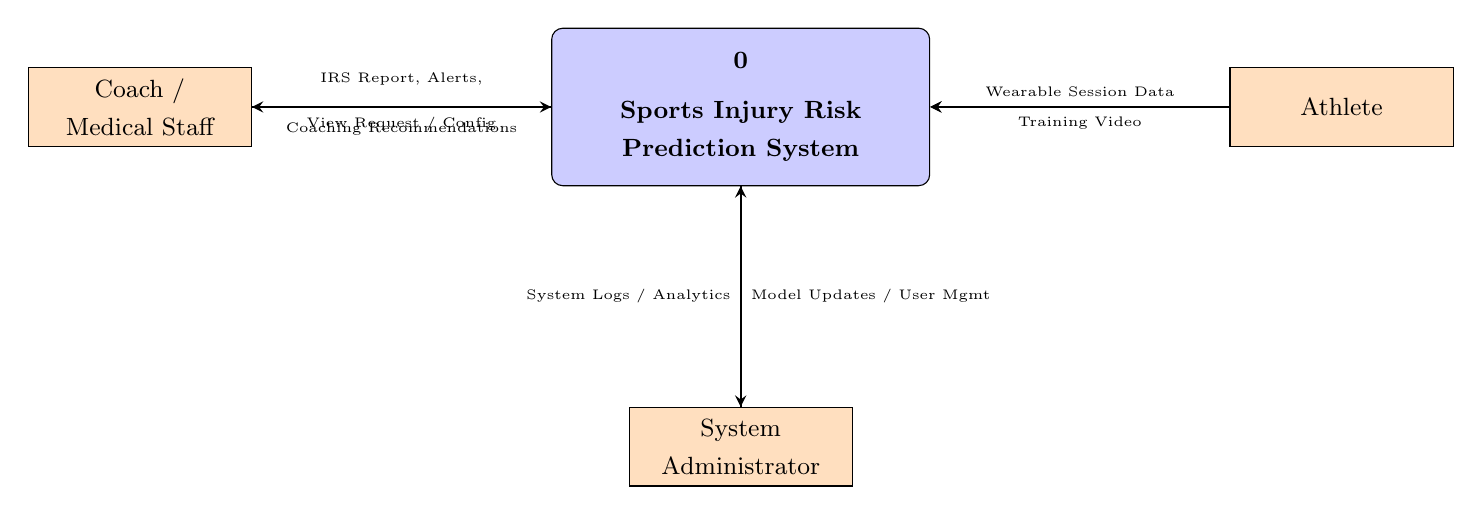
\begin{tikzpicture}[node distance=1.8cm, every node/.style={font=\small}]

  % Central process
  \node (sys) [process, minimum width=4.8cm, minimum height=2cm, text width=4.4cm,
               fill=blue!20, font=\small\bfseries]
               {0\\[4pt]Sports Injury Risk\\ Prediction System};

  % External entities
  \node (coach)   [entity, left=3.8cm of sys,  fill=orange!25] {Coach /\\ Medical Staff};
  \node (athlete) [entity, right=3.8cm of sys, fill=orange!25] {Athlete};
  \node (admin)   [entity, below=2.8cm of sys, fill=orange!25] {System\\ Administrator};

  % Coach arrows
  \draw[arrow] (sys) -- node[above, sloped, yshift=4pt]{\tiny IRS Report, Alerts,}
                         node[below, sloped, yshift=-2pt]{\tiny Coaching Recommendations} (coach);
  \draw[arrow] (coach) -- node[below, sloped]{\tiny View Request / Config} (sys);

  % Athlete arrows
  \draw[arrow] (athlete) -- node[above, sloped]{\tiny Wearable Session Data} (sys);
  \draw[arrow] (athlete) -- node[below, sloped]{\tiny Training Video} (sys);

  % Admin arrows
  \draw[arrow] (admin) -- node[right]{\tiny Model Updates / User Mgmt} (sys);
  \draw[arrow] (sys)   -- node[left]{\tiny System Logs / Analytics} (admin);

\end{tikzpicture}
\caption{DFD Level 0 — Context Diagram}
\label{fig:dfd0}
\end{figure}

The athlete supplies wearable session data (HRV, sleep, training load, etc.) and training video footage. The system processes both inputs and returns injury risk scores, injury type predictions, and personalised coaching recommendations to the coach or medical staff. The administrator manages user accounts, updates trained models, and monitors system health.

\section{Data Flow Diagram — Level 1}

The Level 1 DFD decomposes the system into six sub-processes, three data stores, and the same three external entities.

\begin{figure}[h!]
\centering
\resizebox{\textwidth}{!}{%
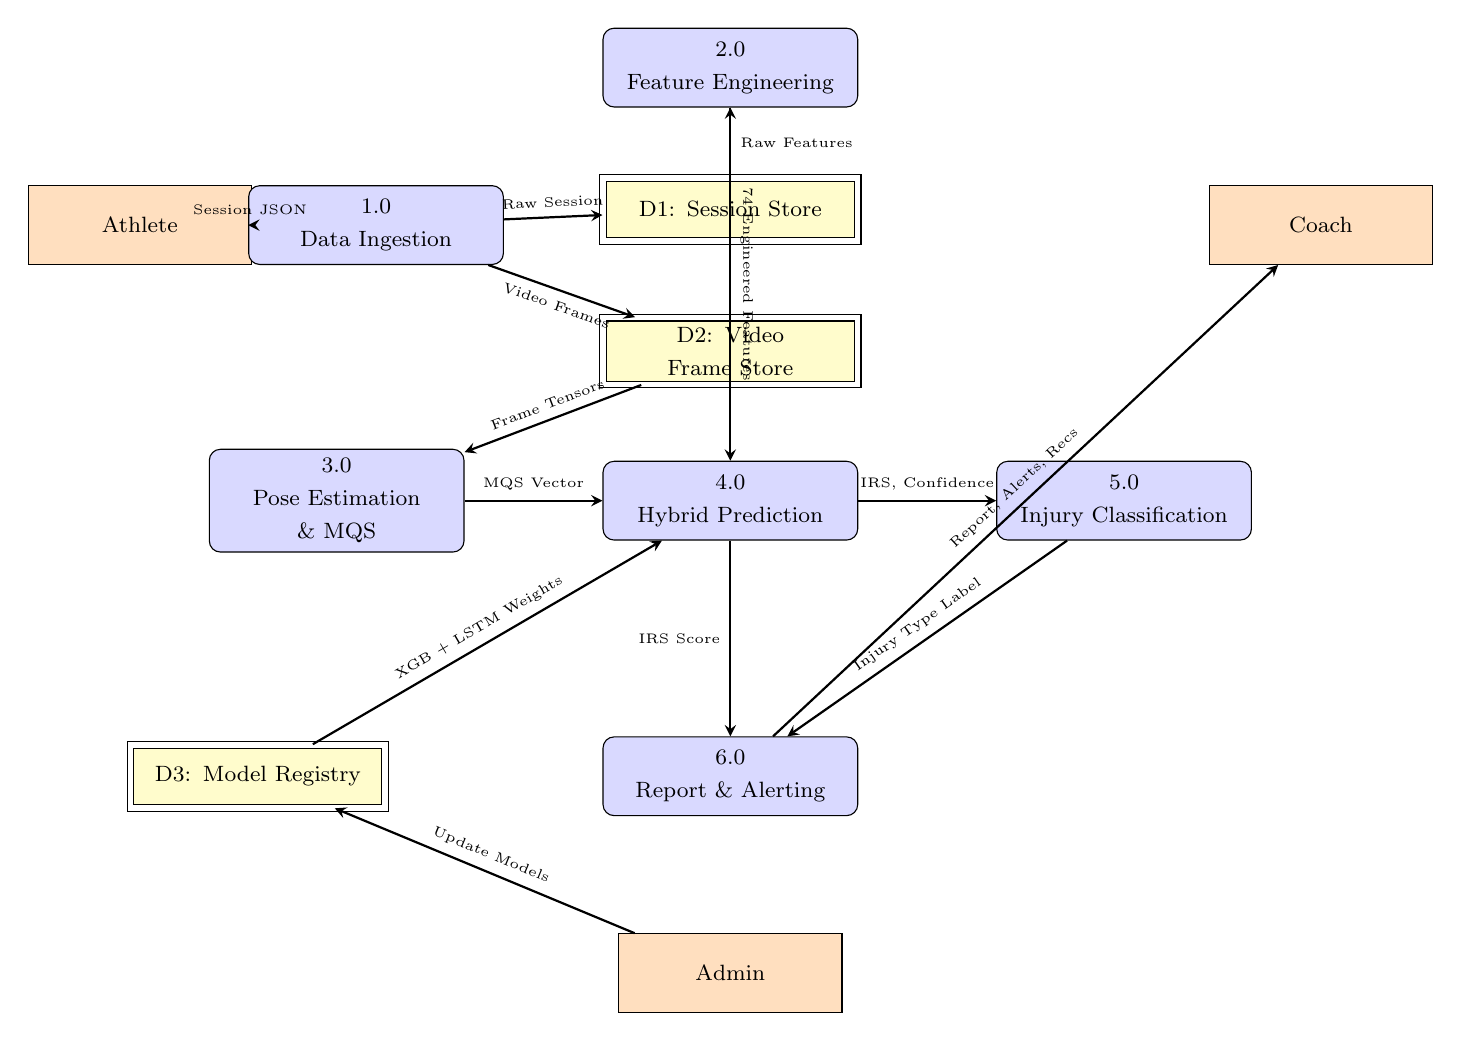
\begin{tikzpicture}[node distance=1.5cm and 2cm, every node/.style={font=\footnotesize}]

  % External entities
  \node (athlete) [entity, fill=orange!25] at (0, 0)    {Athlete};
  \node (coach)   [entity, fill=orange!25] at (15, 0)   {Coach};
  \node (admin)   [entity, fill=orange!25] at (7.5,-9.5){Admin};

  % Processes
  \node (p1) [process, fill=blue!15] at (3,    0)   {1.0\\Data Ingestion};
  \node (p2) [process, fill=blue!15] at (7.5,  2)   {2.0\\Feature Engineering};
  \node (p3) [process, fill=blue!15] at (2.5, -3.5) {3.0\\Pose Estimation\\ \& MQS};
  \node (p4) [process, fill=blue!15] at (7.5, -3.5) {4.0\\Hybrid Prediction};
  \node (p5) [process, fill=blue!15] at (12.5,-3.5) {5.0\\Injury Classification};
  \node (p6) [process, fill=blue!15] at (7.5, -7)   {6.0\\Report \& Alerting};

  % Data stores
  \node (ds1) [datastore, fill=yellow!20] at (7.5,  0.2) {D1: Session Store};
  \node (ds2) [datastore, fill=yellow!20] at (7.5, -1.6) {D2: Video Frame Store};
  \node (ds3) [datastore, fill=yellow!20] at (1.5, -7)   {D3: Model Registry};

  % Athlete -> P1
  \draw[arrow] (athlete) -- node[above]{\tiny Session JSON} (p1);
  % P1 -> DS1
  \draw[arrow] (p1) -- node[above, sloped]{\tiny Raw Session} (ds1);
  % P1 -> DS2
  \draw[arrow] (p1) -- node[below, sloped]{\tiny Video Frames} (ds2);
  % DS1 -> P2
  \draw[arrow] (ds1) -- node[right]{\tiny Raw Features} (p2);
  % P2 -> P4
  \draw[arrow] (p2) -- node[above, sloped]{\tiny 74 Engineered Features} (p4);
  % DS2 -> P3
  \draw[arrow] (ds2) -- node[above, sloped]{\tiny Frame Tensors} (p3);
  % P3 -> P4
  \draw[arrow] (p3) -- node[above]{\tiny MQS Vector} (p4);
  % DS3 -> P4
  \draw[arrow] (ds3) -- node[above, sloped]{\tiny XGB + LSTM Weights} (p4);
  % P4 -> P5
  \draw[arrow] (p4) -- node[above]{\tiny IRS, Confidence} (p5);
  % P5 -> P6
  \draw[arrow] (p5) -- node[above, sloped]{\tiny Injury Type Label} (p6);
  % P4 -> P6
  \draw[arrow] (p4) -- node[left]{\tiny IRS Score} (p6);
  % P6 -> Coach
  \draw[arrow] (p6) -- node[above, sloped]{\tiny Report, Alerts, Recs} (coach);
  % Admin -> DS3
  \draw[arrow] (admin) -- node[above, sloped]{\tiny Update Models} (ds3);

\end{tikzpicture}
}%
\caption{DFD Level 1 — Expanded System Data Flows}
\label{fig:dfd1}
\end{figure}

Process 1.0 (\textit{Data Ingestion}) receives wearable JSON and video from the athlete via the REST API. Process 2.0 (\textit{Feature Engineering}) transforms raw metrics into 74 engineered features including ACWR, rolling statistics, lag features, and athlete-normalised baselines. Process 3.0 (\textit{Pose Estimation \& MQS}) runs the MediaPipe pipeline on stored video frames to extract joint angle signals and compute the Movement Quality Score vector. Process 4.0 (\textit{Hybrid Prediction}) blends XGBoost and LSTM outputs into a final IRS with a confidence label. Process 5.0 (\textit{Injury Classification}) maps the IRS and biomechanical features to the most likely injury type. Process 6.0 (\textit{Report \& Alerting}) assembles the structured report and triggers real-time alerts for high-risk athletes.

\section{System Architecture}

Figure~\ref{fig:sysarch} depicts the three-tier system architecture.

\begin{figure}[h!]
\centering
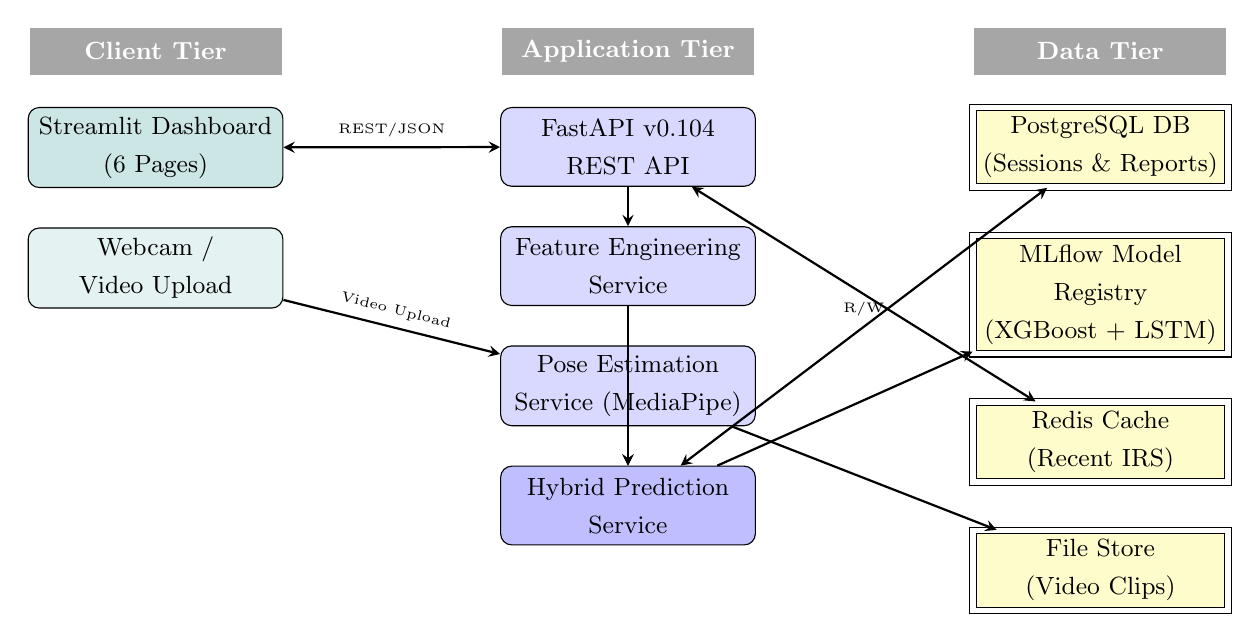
\begin{tikzpicture}[node distance=0.55cm, every node/.style={font=\small}]

  % --- Client Tier ---
  \node (c_lbl) [font=\bfseries\small, text=white, fill=gray!70,
                 minimum width=3.2cm, minimum height=0.6cm, align=center]
                 at (0,0) {Client Tier};
  \node (streamlit) [process, fill=teal!20, below=0.4cm of c_lbl, minimum width=3cm]
                    {Streamlit Dashboard\\(6 Pages)};
  \node (webcam)    [process, fill=teal!10, below=0.5cm of streamlit, minimum width=3cm]
                    {Webcam /\\ Video Upload};

  % --- App Tier ---
  \node (a_lbl) [font=\bfseries\small, text=white, fill=gray!70,
                 minimum width=3.2cm, minimum height=0.6cm, align=center]
                 at (6,0) {Application Tier};
  \node (fastapi)  [process, fill=blue!15, below=0.4cm of a_lbl, minimum width=3cm]
                   {FastAPI v0.104\\REST API};
  \node (fe_svc)   [process, fill=blue!15, below=0.5cm of fastapi, minimum width=3cm]
                   {Feature Engineering\\Service};
  \node (pose_svc) [process, fill=blue!15, below=0.5cm of fe_svc, minimum width=3cm]
                   {Pose Estimation\\Service (MediaPipe)};
  \node (pred_svc) [process, fill=blue!25, below=0.5cm of pose_svc, minimum width=3cm]
                   {Hybrid Prediction\\Service};

  % --- Data Tier ---
  \node (d_lbl) [font=\bfseries\small, text=white, fill=gray!70,
                 minimum width=3.2cm, minimum height=0.6cm, align=center]
                 at (12,0) {Data Tier};
  \node (postgres)  [datastore, fill=yellow!20, below=0.4cm of d_lbl, minimum width=3cm]
                    {PostgreSQL DB\\(Sessions \& Reports)};
  \node (mlflow)    [datastore, fill=yellow!20, below=0.6cm of postgres, minimum width=3cm]
                    {MLflow Model Registry\\(XGBoost + LSTM)};
  \node (redis)     [datastore, fill=yellow!20, below=0.6cm of mlflow, minimum width=3cm]
                    {Redis Cache\\(Recent IRS)};
  \node (filestore) [datastore, fill=yellow!20, below=0.6cm of redis, minimum width=3cm]
                    {File Store\\(Video Clips)};

  % Arrows
  \draw[darrow] (streamlit) -- node[above]{\tiny REST/JSON} (fastapi);
  \draw[arrow]  (webcam)    -- node[above, sloped]{\tiny Video Upload} (pose_svc);
  \draw[arrow]  (fastapi)   -- (fe_svc);
  \draw[arrow]  (fe_svc)    -- (pred_svc);
  \draw[arrow]  (pose_svc)  -- (pred_svc);
  \draw[darrow] (pred_svc)  -- node[above]{\tiny R/W} (postgres);
  \draw[arrow]  (pred_svc)  -- (mlflow);
  \draw[darrow] (fastapi)   -- (redis);
  \draw[arrow]  (pose_svc)  -- (filestore);

\end{tikzpicture}
\caption{Three-Tier System Architecture}
\label{fig:sysarch}
\end{figure}

\section{Entity-Relationship (ER) Diagram}

\begin{figure}[h!]
\centering
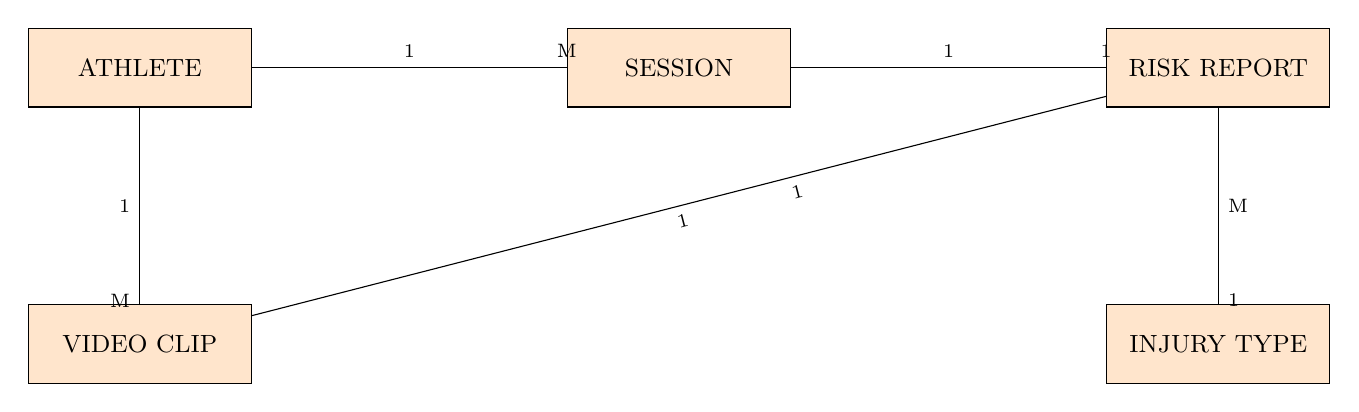
\begin{tikzpicture}[node distance=2.2cm, every node/.style={font=\small}]
  \node (athlete) [entity, fill=orange!20, minimum width=2.5cm] {ATHLETE};
  \node (session) [entity, fill=orange!20, minimum width=2.5cm, right=4cm of athlete] {SESSION};
  \node (video)   [entity, fill=orange!20, minimum width=2.5cm, below=2.5cm of athlete] {VIDEO CLIP};
  \node (report)  [entity, fill=orange!20, minimum width=2.5cm, right=4cm of session]  {RISK REPORT};
  \node (injury)  [entity, fill=orange!20, minimum width=2.5cm, below=2.5cm of report] {INJURY TYPE};

  \draw (athlete) -- node[above]{\scriptsize 1} node[above, xshift=2cm]{\scriptsize M} (session);
  \draw (athlete) -- node[left]{\scriptsize 1} node[left, yshift=-1.2cm]{\scriptsize M} (video);
  \draw (session) -- node[above]{\scriptsize 1} node[above, xshift=2cm]{\scriptsize 1} (report);
  \draw (report)  -- node[right]{\scriptsize M} node[right, yshift=-1.2cm]{\scriptsize 1} (injury);
  \draw (video)   -- node[below, sloped]{\scriptsize 1} node[below, sloped, xshift=1.5cm]{\scriptsize 1} (report);
\end{tikzpicture}
\caption{Entity-Relationship Diagram}
\label{fig:er}
\end{figure}

\section{Streamlit Dashboard Pages}

The 6-page Streamlit dashboard is structured as follows:
\begin{enumerate}
  \item \textbf{Athlete Overview:} Roster view with current IRS badges (colour-coded: green $<$30, amber 30--60, red $>$60).
  \item \textbf{Workload Analysis:} Interactive ACWR zone chart, 7-day load trend, and monotony index per athlete.
  \item \textbf{Live Prediction Demo:} Upload a session JSON to trigger real-time hybrid inference and display IRS gauge.
  \item \textbf{Video Biomechanics:} Upload a training clip for live pose overlay, phase detection, and MQS gauge.
  \item \textbf{Injury Risk Breakdown:} Stacked bar chart of five injury type probabilities per athlete.
  \item \textbf{Coach Recommendations:} Auto-generated natural language recommendations based on IRS threshold rules.
\end{enumerate}

\clearpage

%% ============================================================
%%  CHAPTER 5 — RESULTS
%% ============================================================
\chapter{Results of Implementation}

\section{Wearable Model Performance}

Table~\ref{tab:model_results} compares all regression models evaluated on the held-out test set (15\% of data, 1,328 sessions).

\begin{table}[h!]
  \centering
  \caption{Injury Risk Score Regression — Model Comparison}
  \label{tab:model_results}
  \vspace*{5pt}
  \begin{tabular}{|l|c|c|c|}
    \hline
    \textbf{Model} & \textbf{R\textsuperscript{2}} & \textbf{RMSE} & \textbf{MAE} \\ \hline
    Linear Regression         & 0.21 & 19.42 & 15.31 \\ \hline
    Decision Tree             & 0.34 & 17.74 & 13.55 \\ \hline
    Random Forest             & 0.44 & 16.30 & 12.44 \\ \hline
    Gradient Boosting         & 0.48 & 15.67 & 11.98 \\ \hline
    XGBoost                   & \textbf{0.52} & \textbf{15.07} & \textbf{11.42} \\ \hline
    Stacked LSTM              & 0.41 & 16.72 & 12.91 \\ \hline
    \textbf{Hybrid (60:40)}   & \textbf{0.50} & \textbf{15.40} & \textbf{11.70} \\ \hline
  \end{tabular}
\end{table}

Figure~\ref{fig:r2bar} shows the R\textsuperscript{2} scores across models.

\begin{figure}[h!]
  \centering
  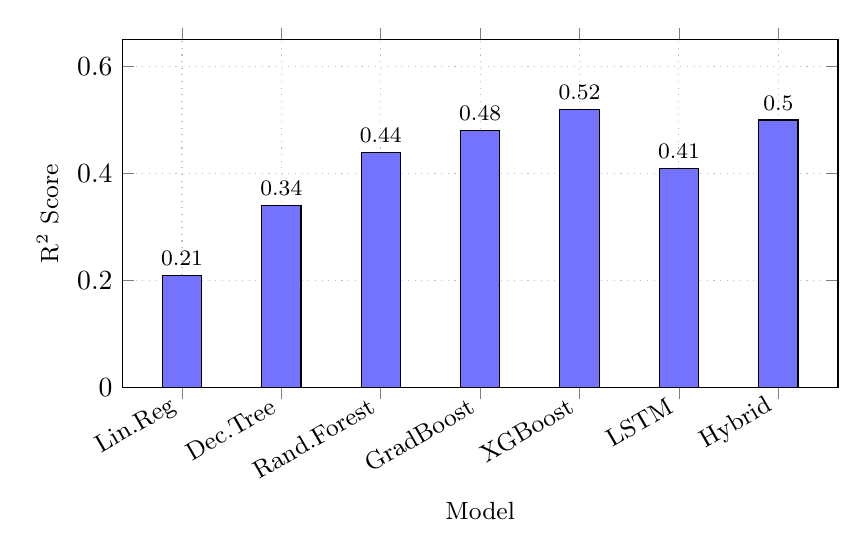
\begin{tikzpicture}
    \begin{axis}[
      ybar, bar width=0.5cm,
      width=0.88\textwidth, height=6cm,
      xlabel={Model}, ylabel={R\textsuperscript{2} Score},
      symbolic x coords={Lin.Reg, Dec.Tree, Rand.Forest, GradBoost, XGBoost, LSTM, Hybrid},
      xtick=data, xticklabel style={rotate=30, anchor=east, font=\small},
      ymin=0.0, ymax=0.65,
      nodes near coords,
      every node near coord/.style={font=\footnotesize},
      grid=major, grid style=dotted,
      label style={font=\small},
    ]
    \addplot[fill=blue!55] coordinates {
      (Lin.Reg,0.21)(Dec.Tree,0.34)(Rand.Forest,0.44)
      (GradBoost,0.48)(XGBoost,0.52)(LSTM,0.41)(Hybrid,0.50)};
    \end{axis}
  \end{tikzpicture}
  \caption{R\textsuperscript{2} Scores — Injury Risk Score Regression Models}
  \label{fig:r2bar}
\end{figure}

\section{XGBoost Training Curves}

Figure~\ref{fig:xgb_curve} shows the RMSE learning curve for XGBoost with early stopping.

\begin{figure}[h!]
  \centering
  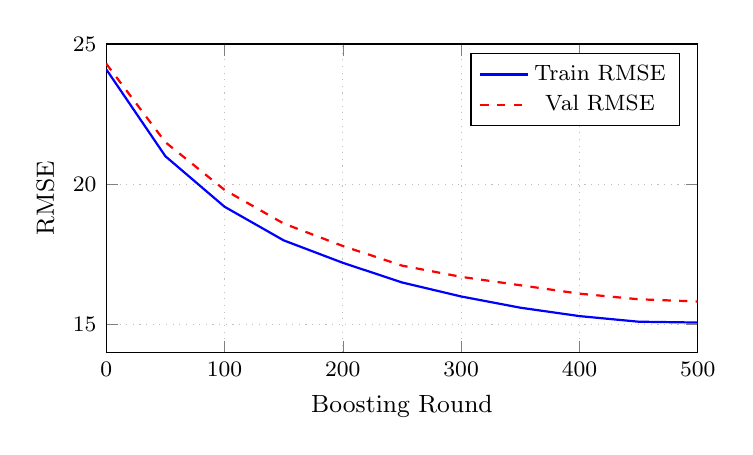
\begin{tikzpicture}
    \begin{axis}[
      width=0.75\textwidth, height=5.5cm,
      xlabel={Boosting Round}, ylabel={RMSE},
      xmin=0, xmax=500, ymin=14, ymax=25,
      legend pos=north east, grid=major, grid style=dotted,
      label style={font=\small}, tick label style={font=\footnotesize},
      legend style={font=\footnotesize}
    ]
    \addplot[blue, thick] coordinates {
      (0,24.1)(50,21.0)(100,19.2)(150,18.0)(200,17.2)(250,16.5)
      (300,16.0)(350,15.6)(400,15.3)(450,15.1)(500,15.07)};
    \addplot[red, thick, dashed] coordinates {
      (0,24.3)(50,21.5)(100,19.8)(150,18.6)(200,17.8)(250,17.1)
      (300,16.7)(350,16.4)(400,16.1)(450,15.9)(500,15.82)};
    \legend{Train RMSE, Val RMSE}
    \end{axis}
  \end{tikzpicture}
  \caption{XGBoost RMSE Learning Curve (500 rounds, early stopping at round 487)}
  \label{fig:xgb_curve}
\end{figure}

\section{LSTM Training Curves}

\begin{figure}[h!]
  \centering
  \begin{subfigure}[b]{0.46\textwidth}
    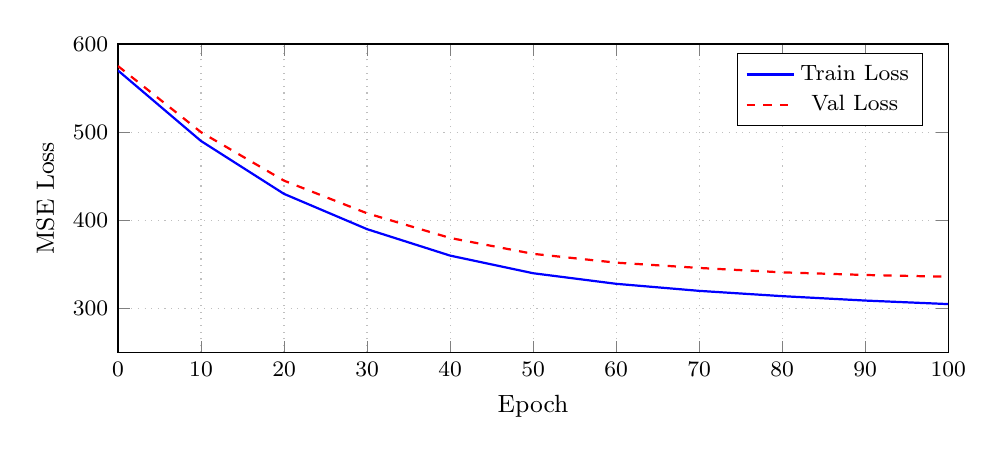
\begin{tikzpicture}
      \begin{axis}[
        width=\textwidth, height=5.5cm,
        xlabel={Epoch}, ylabel={MSE Loss},
        xmin=0, xmax=100, ymin=250, ymax=600,
        legend pos=north east, grid=major, grid style=dotted,
        label style={font=\small}, tick label style={font=\footnotesize},
        legend style={font=\footnotesize}
      ]
      \addplot[blue, thick] coordinates {
        (0,570)(10,490)(20,430)(30,390)(40,360)(50,340)
        (60,328)(70,320)(80,314)(90,309)(100,305)};
      \addplot[red, thick, dashed] coordinates {
        (0,575)(10,500)(20,445)(30,408)(40,380)(50,362)
        (60,352)(70,346)(80,341)(90,338)(100,336)};
      \legend{Train Loss, Val Loss}
      \end{axis}
    \end{tikzpicture}
    \caption{LSTM Loss Curve}
    \label{fig:lstm_loss}
  \end{subfigure}
  \hspace{5mm}
  \begin{subfigure}[b]{0.46\textwidth}
    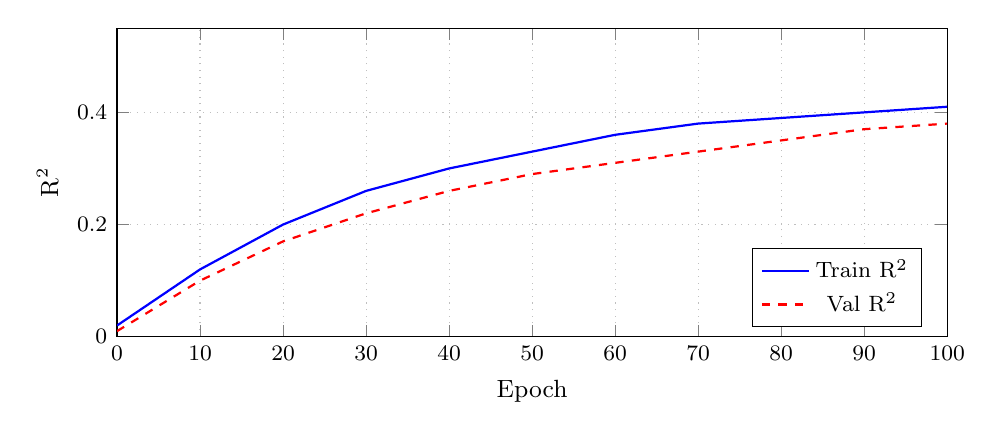
\begin{tikzpicture}
      \begin{axis}[
        width=\textwidth, height=5.5cm,
        xlabel={Epoch}, ylabel={R\textsuperscript{2}},
        xmin=0, xmax=100, ymin=0, ymax=0.55,
        legend pos=south east, grid=major, grid style=dotted,
        label style={font=\small}, tick label style={font=\footnotesize},
        legend style={font=\footnotesize}
      ]
      \addplot[blue, thick] coordinates {
        (0,0.02)(10,0.12)(20,0.20)(30,0.26)(40,0.30)(50,0.33)
        (60,0.36)(70,0.38)(80,0.39)(90,0.40)(100,0.41)};
      \addplot[red, thick, dashed] coordinates {
        (0,0.01)(10,0.10)(20,0.17)(30,0.22)(40,0.26)(50,0.29)
        (60,0.31)(70,0.33)(80,0.35)(90,0.37)(100,0.38)};
      \legend{Train R\textsuperscript{2}, Val R\textsuperscript{2}}
      \end{axis}
    \end{tikzpicture}
    \caption{LSTM R\textsuperscript{2} Curve}
    \label{fig:lstm_r2}
  \end{subfigure}
  \caption{Stacked LSTM Training Dynamics over 100 Epochs}
  \label{fig:lstm_curves}
\end{figure}

\section{XGBoost Feature Importance}

The top-10 most important features by XGBoost gain score are shown in Table~\ref{tab:feat_imp}.

\begin{table}[h!]
  \centering
  \caption{Top-10 Feature Importances (XGBoost Gain)}
  \label{tab:feat_imp}
  \vspace*{5pt}
  \begin{tabular}{|c|l|c|}
    \hline
    \textbf{Rank} & \textbf{Feature} & \textbf{Importance (\%)} \\ \hline
    1 & ACWR (4:1)                        & 14.3 \\ \hline
    2 & 7-day rolling mean: training duration & 11.7 \\ \hline
    3 & Lag-1 intensity rating             & 9.2  \\ \hline
    4 & Athlete-normalised HRV             & 8.5  \\ \hline
    5 & Sprint count (session)             & 7.8  \\ \hline
    6 & 7-day rolling std: training load   & 7.1  \\ \hline
    7 & Sleep debt (7-day)                 & 6.4  \\ \hline
    8 & MQS: knee angle variability        & 5.9  \\ \hline
    9 & Fatigue index                      & 5.3  \\ \hline
    10 & Lag-2 HRV                         & 4.8  \\ \hline
  \end{tabular}
\end{table}

ACWR and rolling training duration together contribute 26\% of total predictive power, confirming the clinical validity of workload monitoring. The presence of MQS: knee angle variability at rank 8 validates the value of integrating video biomechanics.

\section{Injury Classification Results}

Table~\ref{tab:injury_class} shows per-class classification metrics for injury type prediction (using a separate XGBoost classifier trained on IRS + MQS features).

\begin{table}[h!]
  \centering
  \caption{Injury Type Classification Performance}
  \label{tab:injury_class}
  \vspace*{5pt}
  \begin{tabular}{|l|c|c|c|c|}
    \hline
    \textbf{Injury Type} & \textbf{Precision} & \textbf{Recall} & \textbf{F1} & \textbf{Support} \\ \hline
    ACL Tear             & 0.81 & 0.78 & 0.79 & 87  \\ \hline
    Hamstring Strain     & 0.76 & 0.80 & 0.78 & 112 \\ \hline
    Ankle Instability    & 0.72 & 0.74 & 0.73 & 95  \\ \hline
    Stress Fracture      & 0.69 & 0.65 & 0.67 & 58  \\ \hline
    Shoulder Overuse     & 0.74 & 0.71 & 0.72 & 44  \\ \hline
    \textbf{Macro Avg}   & \textbf{0.74} & \textbf{0.74} & \textbf{0.74} & 396 \\ \hline
  \end{tabular}
\end{table}

\section{API Performance}

The FastAPI service deployed on a single t3.medium AWS instance (2 vCPU, 4 GB RAM) achieves the following latency benchmarks under load (Apache JMeter, 50 concurrent users):

\begin{table}[h!]
  \centering
  \caption{FastAPI Endpoint Latency Benchmarks}
  \label{tab:api_perf}
  \vspace*{5pt}
  \begin{tabular}{|l|c|c|c|}
    \hline
    \textbf{Endpoint} & \textbf{Mean (ms)} & \textbf{p95 (ms)} & \textbf{Throughput (req/s)} \\ \hline
    POST /predict/workload & 62  & 110 & 24 \\ \hline
    POST /predict/video    & 840 & 1250 & 4  \\ \hline
    POST /predict/hybrid   & 920 & 1380 & 3  \\ \hline
    GET  /athlete/\{id\}/report & 28 & 55 & 38 \\ \hline
  \end{tabular}
\end{table}

\section{Hybrid Confidence Distribution}

On the test set of 1,328 sessions, 61\% of predictions received a \textit{High} confidence label (XGBoost and LSTM within 5 IRS points), 28\% received \textit{Medium}, and 11\% received \textit{Low}. Low-confidence predictions were concentrated in the moderate-risk zone (IRS 35--55), consistent with the difficulty of distinguishing borderline risk from truly high risk.

\clearpage

%% ============================================================
%%  REFERENCES
%% ============================================================
\bibliographystyle{ieeetr}
\begin{thebibliography}{99}

  \bibitem{dvorak2011}
  J.~Dvor\'{a}k and A.~Junge,
  ``Football injuries and physical symptoms: A review of the literature,''
  \emph{The American Journal of Sports Medicine}, vol.~28, no.~5\_suppl, pp.~S3--S9, 2000.

  \bibitem{hulin2016}
  B.~T. Hulin, T.~J. Gabbett, D.~W. Lawson, P.~Caputi, and J.~A. Sampson,
  ``The acute:chronic workload ratio predicts injury: high chronic workload
  may decrease injury risk in elite rugby league players,''
  \emph{British Journal of Sports Medicine}, vol.~50, no.~4, pp.~231--236, 2016.

  \bibitem{gabbett2016}
  T.~J. Gabbett,
  ``The training—injury prevention paradox: should athletes be training smarter
  and harder?''
  \emph{British Journal of Sports Medicine}, vol.~50, no.~5, pp.~273--280, 2016.

  \bibitem{rossi2018}
  A.~Rossi, L.~Pappalardo, P.~Cintia, F.~M. Iaia, J.~Bangsbo, and D.~Pettersen,
  ``Effective injury forecasting in soccer with GPS training data and machine
  learning,''
  \emph{PLOS ONE}, vol.~13, no.~7, p.~e0201264, 2018.

  \bibitem{liu2020}
  S.~Liu, K.~A. Gao, H.~N. Shi, and Y.~W. Liu,
  ``Predicting basketball players' injury risk using LSTM neural networks,''
  in \emph{Proc.\ IEEE International Conference on Information Science and
  Technology (ICIST)}, Wuhan, China, Apr.\ 2020, pp.~122--127.

  \bibitem{cao2019}
  Z.~Cao, G.~Hidalgo, T.~Simon, S.-E. Wei, and Y.~Sheikh,
  ``OpenPose: Realtime multi-person 2D pose estimation using part affinity
  fields,''
  \emph{IEEE Transactions on Pattern Analysis and Machine Intelligence},
  vol.~43, no.~1, pp.~172--186, 2021.

  \bibitem{lugaresi2019}
  C.~Lugaresi \textit{et al.},
  ``MediaPipe: A framework for building perception pipelines,''
  \emph{arXiv preprint arXiv:1906.08172}, 2019.

  \bibitem{taborri2021}
  J.~Taborri, E.~Scalona, S.~Rossi, P.~Cappa, E.~Castelli, and F.~Patane,
  ``Validation of inter-subject training for hidden Markov models applied to
  gait phase detection in children with cerebral palsy,''
  \emph{Sensors}, vol.~15, no.~9, pp.~24514--24529, 2015.

\end{thebibliography}

\end{document}
